%----------------------------------------------------------------------------
\chapter{\bevezetes}
%----------------------------------------------------------------------------

I am very passionate about artificial intelligence and as much inspired by the
work of tech companies such as Tesla. Tesla has managed create cutting edge
technology, creating compelling and practical electric cars combined with their
Tesla Autopilot system. It has become iconic to sit in a Tesla and watch it
drive itself. Tesla has already driven 3 billion drives on autopilot, their
access to data is most likely number one in the world. There are other important
companies who develop autopilot systems, one of them is MobilEye an Israeli
subsidiary of Intel corporation that was actually a supplier of Tesla until they
set apart in part due to disagreements on how the technology should be built,
which is an important topic that I will talk about.

There are a couple of topics we should establish first. The first being levels
of autopilot systems as defined by SAE (Society of Automotive Engineers)
(\refstruc{fig:J3016}). 

\begin{figure}[!ht]
    \centering
    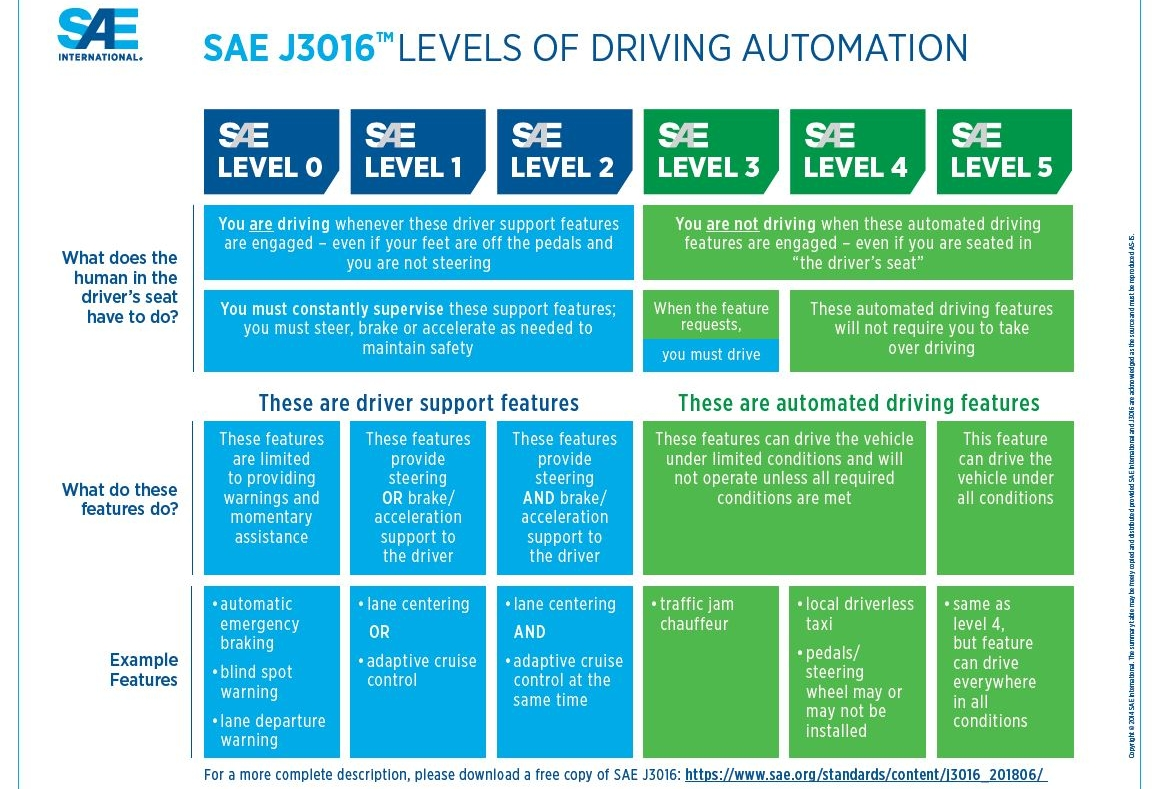
\includegraphics[width=150mm, keepaspectratio]{figures/levels-of-ad.jpg}
    \caption{Levels of driving automation defined in SAE J3016 \cite{j3016b}}
    \label{fig:J3016}
\end{figure}

From level 0 to 2 are automations where the human is still required to fully
monitor the driving environment. Tesla's autopilot is Level 2 which is partial
automation that includes control of steering and both acceleration and
deceleration. From Level 3 the human is not required to monitor the environment.
Full automation, where the driver is not expected to intervene and the vehicle
is able to handle all situations is on Level 5. In order to achieve that level
the autopilot must fully understand the environment.

This is however very difficult. The algorithms that we know today are not enough
to achieve understanding of the environment yet. Even Convolutional Neural
Networks (CNNs) are not cabale of understanding deep concepts of the world. CNNs
are mainly used in computer vision and are useful when we want to recognize
patterns that appear anywhere in 2D images. Today we are able to calssify
images, detect and localize objects, segment images to very high accuracy,
however this doesn't mean the computer \emph{understands} the scenes.
Furthermore these algorithms are trained very specifically: To build a detection
neural network (NN) first a meticulous dataset must be created that tells the
algorithm what must be detected - we call this the ground truth, or training
data set. Then the NN must be trained and optimized until it yields a low error
on the test dataset. We call this Deep Learning due to the fact that the
networks contain millions of parameters that are trained through hundreds of
thousands of iterations. This is not close to what might be general AI.

In this sense we can argue about the meaning of "scene understanding". There is
research going on in the direction of general AI most notably in my opinion by
Yann LeCun the chief at Facebook AI and professsor at NYU, who works a concept
called energy-based models. The Energy-based model that is a form of generative
model allow a mathematical "bounding" or "learning" of a data distribution in
any dimension. Upon prediciton the model tries to generate a possible future for
the current model in time, where the generated future model acts as the
prediciton itself. Generative adversarial networks are a type of these models.
This is in contrast to the other main machine learning approach that is the
discriminative model which is what we use mostly. Perceptrons such as NNs and
CNNs, support vector machines fall into this category, however the distinction
is not clear.

For the purpouse of this thesis hence it is important to define what a system
capabale of understanding scences in driving situations means. The essentials
are the following:
\begin{itemize}
    \item Lane  and path detection
    \item Driveable area detection
    \item Object detection: cars, pedestrians, etc.
    \item Object localization in 3D real world space
    \item Object tracking and identification
    \item Foreign object detection: anything that shouldn't be where it is
    \item Traffic light and sign understanding
    \item Handling occlusion of objects
    \item Pedestrian crossing detection
    \item Knowledge of surroundings and road for example with the help of high
          definition maps
\end{itemize}

In an ideal world, where all cars are autonomous these perceptions would be
enough, however the future of self-driving cars is going to be a transition,
where both humans and machines will drive on the roads. We humans already
account for each other (we try as we can), but self-driving cars will have to
account for us too. We might not be smart but driving on the road sometimes
requires improvization to save a situation and we might need a more general AI.

For the vehicle to understand it's surroundigs first of all it needs sensors.
Each company goes differently about the sensor suite, and it is quite
interesting to examine each solution. I will talk about this in the next
chapter, Related works.

\section{Proposed solution}

As we said to develop our system first of all we need data. There are a lot of
datasets available on the internet for car driving. They include object
detections, segmentations, map data, lidar data. Some of the most notable ones
are the nuScenes dataset\footnote{nuScenes dataset
\url{https://www.nuscenes.org/}}, Waymo dataset\footnote{Waymo dataset
\url{https://waymo.com/open/}} from Google's self-driving car company or the
Cityscapes dataset\footnote{Cityscapes dataset
\url{https://www.cityscapes-dataset.com/}} and more. Each of these datasets are
very good, however they are not really helpful for our case.

In order to localize objects in 3D space I use stereo imaging. Each AD system
today employs stereo camera setting because it is a very simple and cheap but
accurate way of estimating depth for each pixel in an image. In order to have
the \emph{freedom} to create a custom camera setting I cannot rely on these
datasets. Furthermore, I want to measure the success rate of my detector however
there is no dataset that contains all the necessary information, because in fact
it is not possible to collect everything from the real world.

This is why I choose to use a \emph{simulation} instead to test the system.
Using a simulation gives a huge ammount of freedom. My research work started
in looking for simulators that let me extract data from the simulation in each
frame and let's me create custom world scenario and sensor settings. 

After an extensive research of self-driving car simulators of I found CARLA
Simulator\footnote{CARLA Sim \url{http://carla.org/}} \cite{Dosovitskiy17} (a
screenshot is seen on \refstruc{fig:carla}) to be the most advanced one that is
also opensource. CARLA is a quite mature simulator with an API that
fulfills our requirements.

\begin{figure}[!ht]
    \centering
    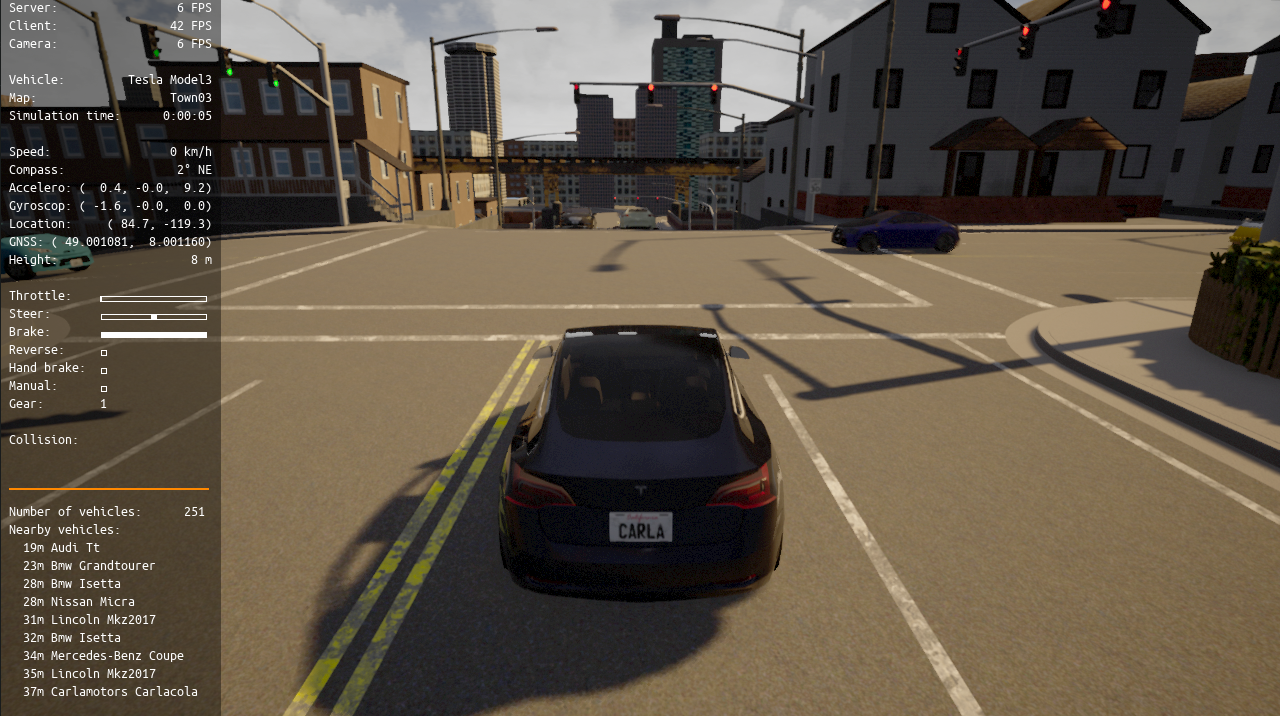
\includegraphics[width=150mm, keepaspectratio]{figures/carla.png}
    \caption{A screenshot from CARLA}
    \label{fig:carla}
\end{figure}

I set up the virtual vehcile with 10 RGB cameras mounted on the roof creating 4
stereo sides as shown on \refstruc{fig:3dmodel2}. As the title of the thesis
says, I only used RGB cameras and no other sensors. This is a similar approach
to what Tesla is taking, except for the radar sensors, contrary to almost all
other players in the field who also employ a Lidar sensor for depth data
including MobilEye and Waymo. Lidar data is good for correction, but it is
better if the AI can equally perform using only RGB cameras, since it is a more
general solution that is closer to how we humans percieve the environment.

\begin{figure}[!ht]
    \centering
    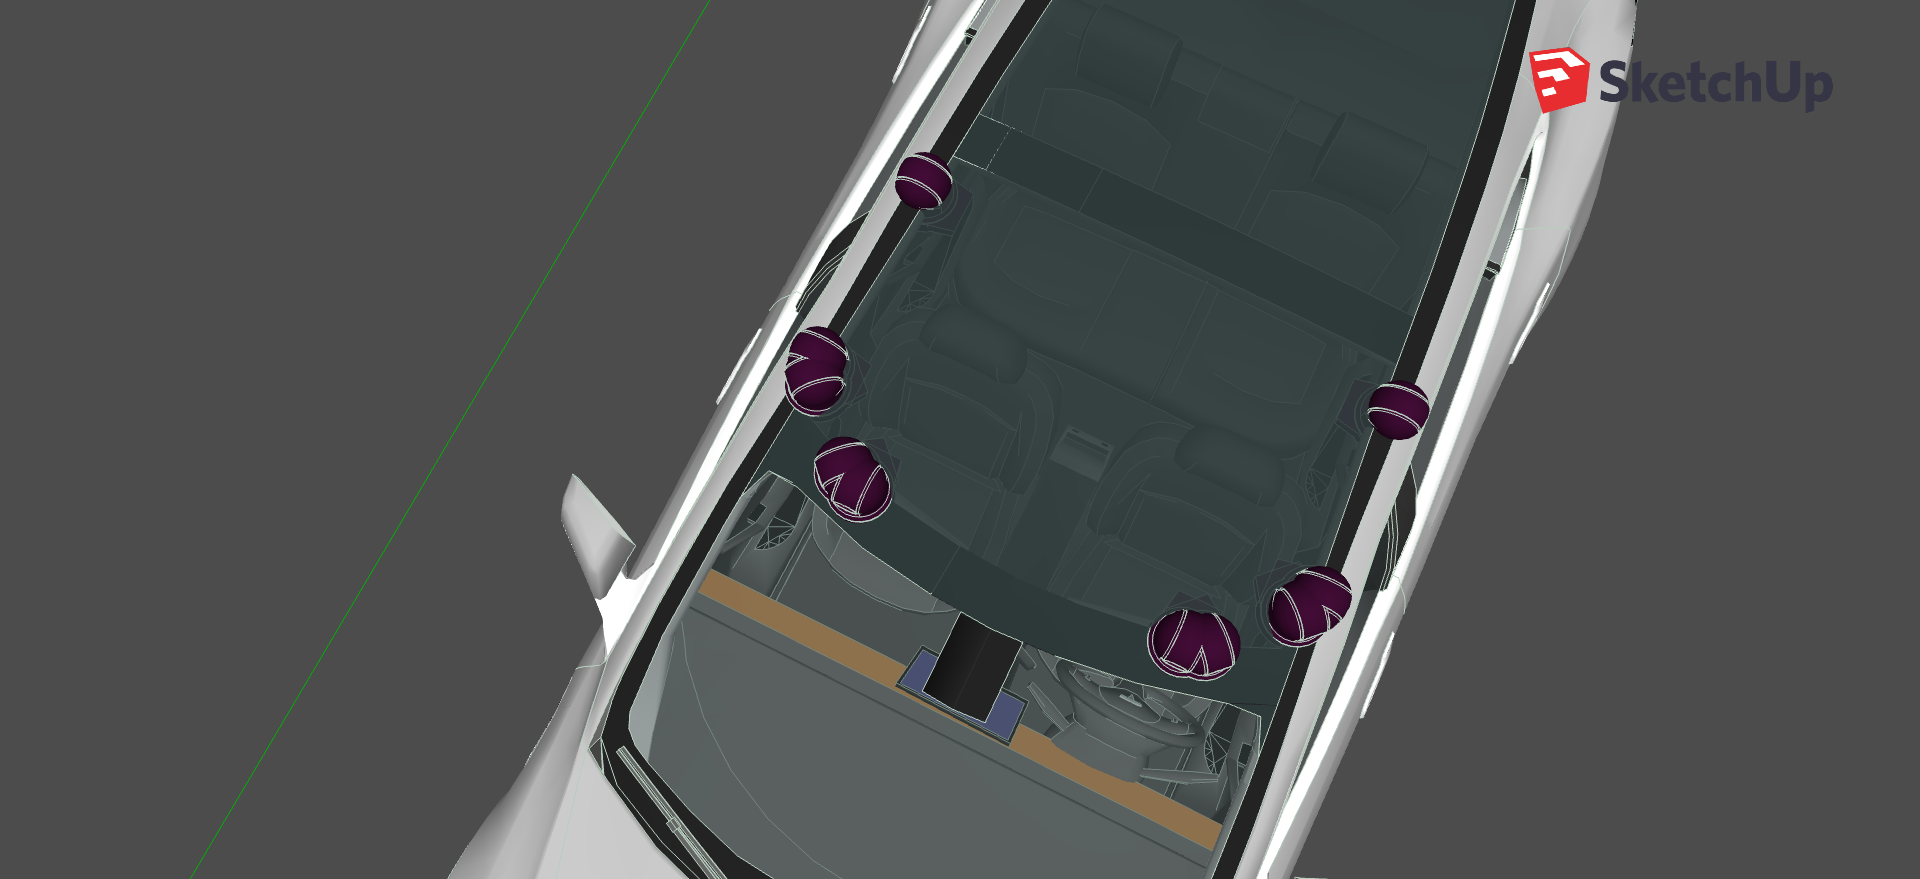
\includegraphics[width=150mm, keepaspectratio]{figures/3dmodel2.png}
    \caption{How the cameras are set up on the roof}
    \label{fig:3dmodel2}
\end{figure}

The detector uses state-of-the-art detection, localization and segmentation model
Detectron2 \cite{wu2019detectron2} a MASK R-CNN conv net model based on Residual
neural networks and Feature Pyramid Networks trained on the COCO general
dataset\footnote{COCO dataset \url{http://cocodataset.org/}}.

Finally I develop a 3D webvisualizer that lets us replay the ground truth and
detection log simultaneously and compare the error between the two.

\refstruc{fig:flow} depicts this taskflow.

\begin{figure}[!ht]
    \centering
    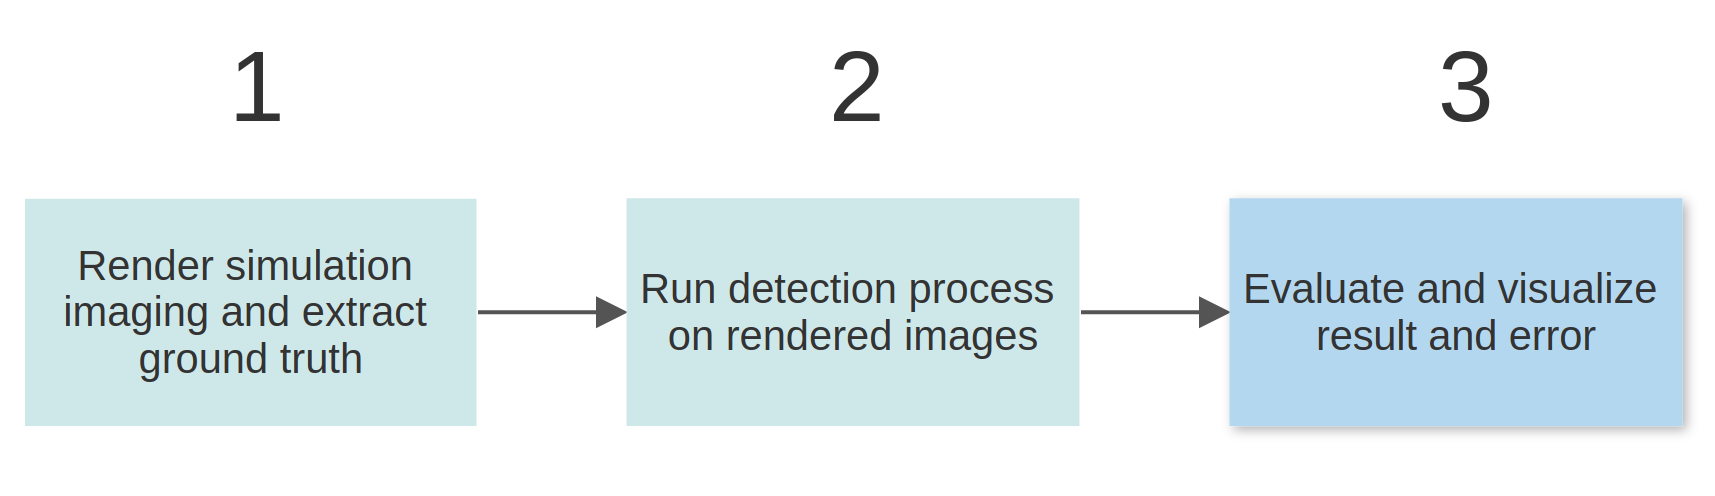
\includegraphics[width=150mm, keepaspectratio]{figures/flowchart.png}
    \caption{Task flow}
    \label{fig:flow}
\end{figure}

\section{Summary of results}

The result is a detector that is capable of localizing vehicles, and pedestrians
on the road up to 100 meters with an accuracy of ~50cm in an angle of 270\degree
centered to the front. The algorithm is written in Python and uses PyTorch, with that on
an NVIDIA Titan X GPU the detector can perform in 2.7FPS for one side, ie. for
two cameras. In an embedded optimized system using C or C++ code this can easily
be improved to even 60FPS creating a real-time system. The code cannot perform
lane detection yet, but that would have been the easier part. The webvisualizer
let's us relplay the simulation frame by frame and see the detection error for
each actor in the scene. It also shows a montage the original, detection and
depthmap. Below, \refstruc{fig:webviz1} shows a screenshot of the webvisualizer
in action.

\begin{figure}[!ht]
    \centering
    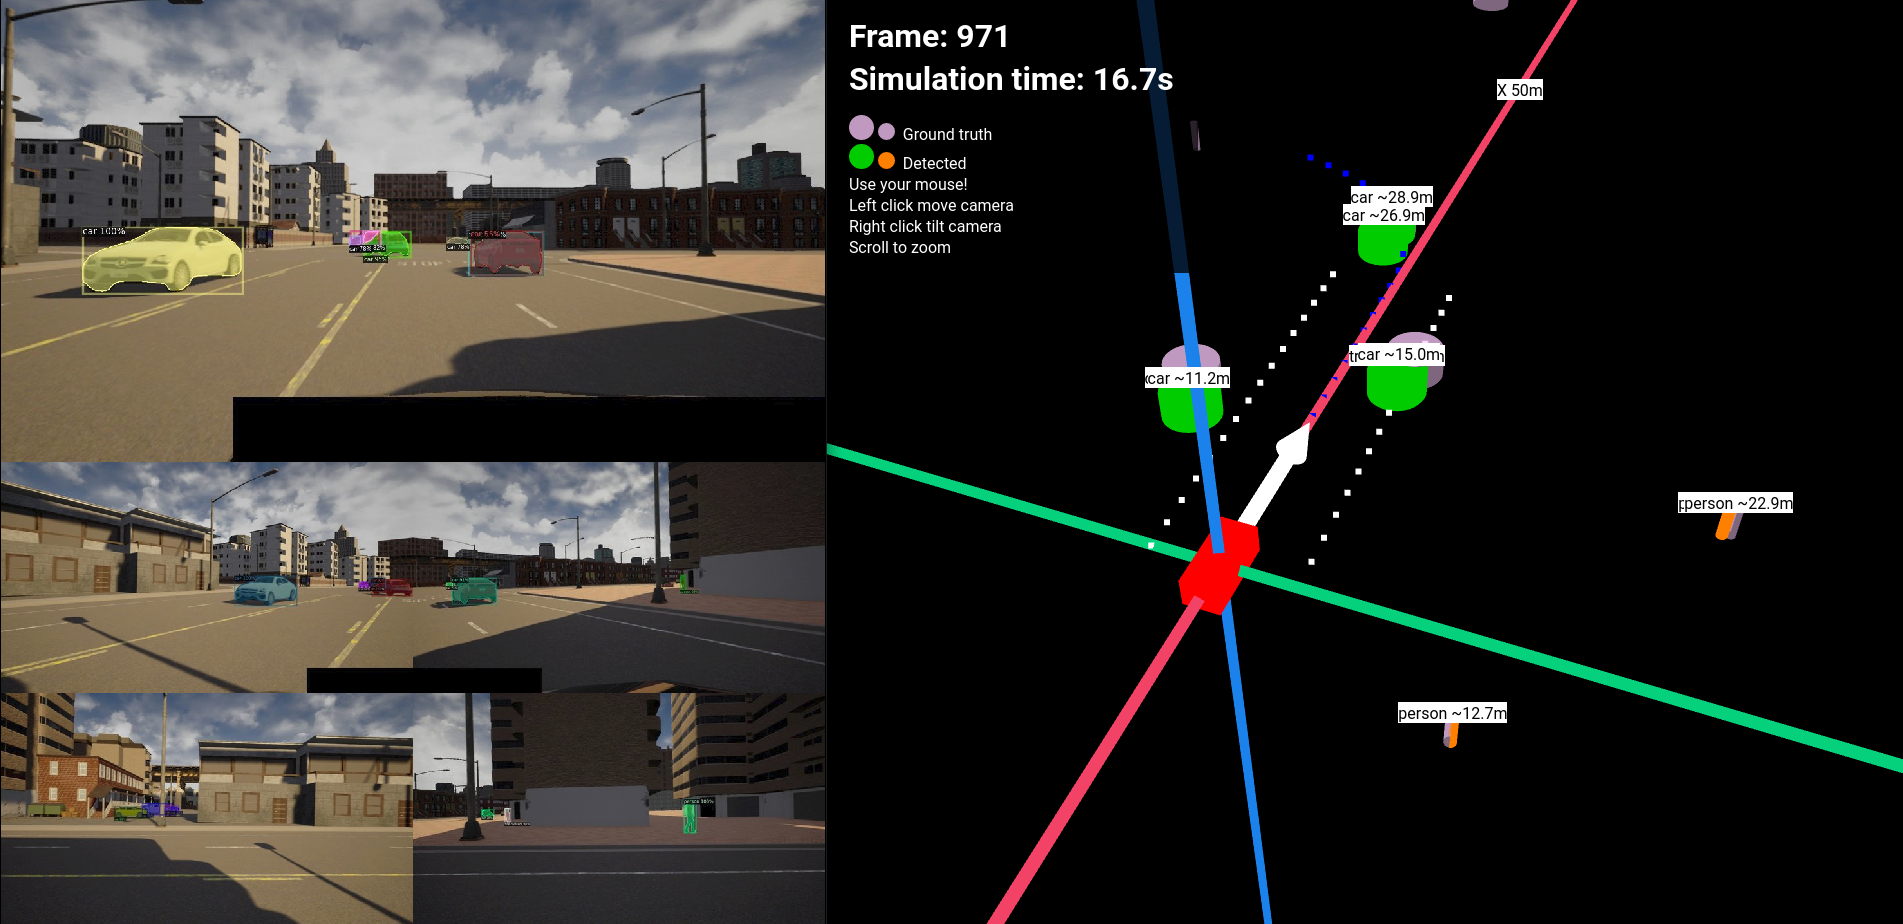
\includegraphics[width=150mm, keepaspectratio]{figures/webviz2.png}
    \caption{3D wevisualizer}
    \label{fig:webviz1}
\end{figure}

All of the code for the thesis, detector, simulator configuration and
webvisualizer is available on \url{https://github.com/najibghadri/msc-thesis}
and you can access the webvisualizer and interactively replay and test
simulations on \url{https://najibghadri.com/msc-thesis/}.


\section{Thesis structure}

In \autoref{chap:sensors} I give an overview of the widely used sensors for
peception in the automotive industry: RGB cameras, radar, Lidar and ultrasonic
sensors. In \autoref{chap:perceptions} I talk about different kinds of
perceptions, state-of-the-art Convolutional Networks and computer vision
algorithms that are useful for our use-case.

In \autoref{chap:relatedwork}, I analyze and compare different self-driving  car
solutions: Tesla and Waymo self-driving cars and MobilEye autopilot. In
\autoref{chap:carlasim}, I introduce CARLA Simulator and some notable features
of it.

In \autoref{chap:assumptions} I define the technical assumptions that I made in
order to simplify the task and the resulting limitations.

\autoref{chap:designimplementation} introduces the Carla simulator details the
design and implementation of the simulator configuration, the detector algorithm
and the webvisualizer.

Then in \autoref{chap:results} I present different measurements and results, and
in \autoref{chap:experimental} I present experimentations that ended up not
being part of the detection. Finally I discuss ways to improve the system in
\autoref{chap:improvement} and close with a conclusion.